\documentclass[twoside]{book}

% Packages required by doxygen
\usepackage{fixltx2e}
\usepackage{calc}
\usepackage{doxygen}
\usepackage[export]{adjustbox} % also loads graphicx
\usepackage{graphicx}
\usepackage[utf8]{inputenc}
\usepackage{makeidx}
\usepackage{multicol}
\usepackage{multirow}
\PassOptionsToPackage{warn}{textcomp}
\usepackage{textcomp}
\usepackage[nointegrals]{wasysym}
\usepackage[table]{xcolor}

% NLS support packages
\usepackage[french]{babel}

% Font selection
\usepackage[T1]{fontenc}
\usepackage[scaled=.90]{helvet}
\usepackage{courier}
\usepackage{amssymb}
\usepackage{sectsty}
\renewcommand{\familydefault}{\sfdefault}
\allsectionsfont{%
  \fontseries{bc}\selectfont%
  \color{darkgray}%
}
\renewcommand{\DoxyLabelFont}{%
  \fontseries{bc}\selectfont%
  \color{darkgray}%
}
\newcommand{\+}{\discretionary{\mbox{\scriptsize$\hookleftarrow$}}{}{}}

% Page & text layout
\usepackage{geometry}
\geometry{%
  a4paper,%
  top=2.5cm,%
  bottom=2.5cm,%
  left=2.5cm,%
  right=2.5cm%
}
\tolerance=750
\hfuzz=15pt
\hbadness=750
\setlength{\emergencystretch}{15pt}
\setlength{\parindent}{0cm}
\setlength{\parskip}{3ex plus 2ex minus 2ex}
\makeatletter
\renewcommand{\paragraph}{%
  \@startsection{paragraph}{4}{0ex}{-1.0ex}{1.0ex}{%
    \normalfont\normalsize\bfseries\SS@parafont%
  }%
}
\renewcommand{\subparagraph}{%
  \@startsection{subparagraph}{5}{0ex}{-1.0ex}{1.0ex}{%
    \normalfont\normalsize\bfseries\SS@subparafont%
  }%
}
\makeatother

% Headers & footers
\usepackage{fancyhdr}
\pagestyle{fancyplain}
\fancyhead[LE]{\fancyplain{}{\bfseries\thepage}}
\fancyhead[CE]{\fancyplain{}{}}
\fancyhead[RE]{\fancyplain{}{\bfseries\leftmark}}
\fancyhead[LO]{\fancyplain{}{\bfseries\rightmark}}
\fancyhead[CO]{\fancyplain{}{}}
\fancyhead[RO]{\fancyplain{}{\bfseries\thepage}}
\fancyfoot[LE]{\fancyplain{}{}}
\fancyfoot[CE]{\fancyplain{}{}}
\fancyfoot[RE]{\fancyplain{}{\bfseries\scriptsize Généré par Doxygen }}
\fancyfoot[LO]{\fancyplain{}{\bfseries\scriptsize Généré par Doxygen }}
\fancyfoot[CO]{\fancyplain{}{}}
\fancyfoot[RO]{\fancyplain{}{}}
\renewcommand{\footrulewidth}{0.4pt}
\renewcommand{\chaptermark}[1]{%
  \markboth{#1}{}%
}
\renewcommand{\sectionmark}[1]{%
  \markright{\thesection\ #1}%
}

% Indices & bibliography
\usepackage{natbib}
\usepackage[titles]{tocloft}
\setcounter{tocdepth}{3}
\setcounter{secnumdepth}{5}
\makeindex

% Hyperlinks (required, but should be loaded last)
\usepackage{ifpdf}
\ifpdf
  \usepackage[pdftex,pagebackref=true]{hyperref}
\else
  \usepackage[ps2pdf,pagebackref=true]{hyperref}
\fi
\hypersetup{%
  colorlinks=true,%
  linkcolor=blue,%
  citecolor=blue,%
  unicode%
}

% Custom commands
\newcommand{\clearemptydoublepage}{%
  \newpage{\pagestyle{empty}\cleardoublepage}%
}

\usepackage{caption}
\captionsetup{labelsep=space,justification=centering,font={bf},singlelinecheck=off,skip=4pt,position=top}

%===== C O N T E N T S =====

\begin{document}

% Titlepage & ToC
\hypersetup{pageanchor=false,
             bookmarksnumbered=true,
             pdfencoding=unicode
            }
\pagenumbering{alph}
\begin{titlepage}
\vspace*{7cm}
\begin{center}%
{\Large Medi\+Watch\+Web\+Site \\[1ex]\large 0.\+0.\+0-\/\+M\+VP }\\
\vspace*{1cm}
{\large Généré par Doxygen 1.8.13}\\
\end{center}
\end{titlepage}
\clearemptydoublepage
\pagenumbering{roman}
\tableofcontents
\clearemptydoublepage
\pagenumbering{arabic}
\hypersetup{pageanchor=true}

%--- Begin generated contents ---
\chapter{Index des espaces de nommage}
\doxysection{Liste des espaces de nommage}
Liste de tous les espaces de nommage documentés avec une brève description\+:\begin{DoxyCompactList}
\item\contentsline{section}{\mbox{\hyperlink{namespace_blazing_blog}{Blazing\+Blog}} }{\pageref{namespace_blazing_blog}}{}
\item\contentsline{section}{\mbox{\hyperlink{namespace_blazing_blog_1_1_server}{Blazing\+Blog.\+Server}} }{\pageref{namespace_blazing_blog_1_1_server}}{}
\item\contentsline{section}{\mbox{\hyperlink{namespace_blazing_blog_1_1_server_1_1_controllers}{Blazing\+Blog.\+Server.\+Controllers}} }{\pageref{namespace_blazing_blog_1_1_server_1_1_controllers}}{}
\item\contentsline{section}{\mbox{\hyperlink{namespace_mediwatch}{Mediwatch}} }{\pageref{namespace_mediwatch}}{}
\item\contentsline{section}{\mbox{\hyperlink{namespace_mediwatch_1_1_server}{Mediwatch.\+Server}} }{\pageref{namespace_mediwatch_1_1_server}}{}
\item\contentsline{section}{\mbox{\hyperlink{namespace_mediwatch_1_1_server_1_1_areas}{Mediwatch.\+Server.\+Areas}} }{\pageref{namespace_mediwatch_1_1_server_1_1_areas}}{}
\item\contentsline{section}{\mbox{\hyperlink{namespace_mediwatch_1_1_server_1_1_areas_1_1_identity}{Mediwatch.\+Server.\+Areas.\+Identity}} }{\pageref{namespace_mediwatch_1_1_server_1_1_areas_1_1_identity}}{}
\item\contentsline{section}{\mbox{\hyperlink{namespace_mediwatch_1_1_server_1_1_areas_1_1_identity_1_1_data}{Mediwatch.\+Server.\+Areas.\+Identity.\+Data}} }{\pageref{namespace_mediwatch_1_1_server_1_1_areas_1_1_identity_1_1_data}}{}
\item\contentsline{section}{\mbox{\hyperlink{namespace_mediwatch_1_1_server_1_1_controllers}{Mediwatch.\+Server.\+Controllers}} \\*Test controller }{\pageref{namespace_mediwatch_1_1_server_1_1_controllers}}{}
\item\contentsline{section}{\mbox{\hyperlink{namespace_mediwatch_1_1_server_1_1_migrations}{Mediwatch.\+Server.\+Migrations}} }{\pageref{namespace_mediwatch_1_1_server_1_1_migrations}}{}
\item\contentsline{section}{\mbox{\hyperlink{namespace_mediwatch_1_1_server_1_1_migrations_1_1_db_context_mediwatch_migrations}{Mediwatch.\+Server.\+Migrations.\+Db\+Context\+Mediwatch\+Migrations}} }{\pageref{namespace_mediwatch_1_1_server_1_1_migrations_1_1_db_context_mediwatch_migrations}}{}
\item\contentsline{section}{\mbox{\hyperlink{namespace_mediwatch_1_1_server_1_1_pages}{Mediwatch.\+Server.\+Pages}} }{\pageref{namespace_mediwatch_1_1_server_1_1_pages}}{}
\item\contentsline{section}{\mbox{\hyperlink{namespace_mediwatch_1_1_server_1_1_ressources}{Mediwatch.\+Server.\+Ressources}} }{\pageref{namespace_mediwatch_1_1_server_1_1_ressources}}{}
\item\contentsline{section}{\mbox{\hyperlink{namespace_server}{Server}} }{\pageref{namespace_server}}{}
\item\contentsline{section}{\mbox{\hyperlink{namespace_server_1_1_utils}{Server.\+Utils}} }{\pageref{namespace_server_1_1_utils}}{}
\end{DoxyCompactList}

\chapter{Index hiérarchique}
\section{Hiérarchie des classes}
Cette liste d\textquotesingle{}héritage est classée approximativement par ordre alphabétique \+:\begin{DoxyCompactList}
\item Controller\begin{DoxyCompactList}
\item \contentsline{section}{Mediwatch.\+Server.\+Controllers.\+Email\+Controller}{\pageref{class_mediwatch_1_1_server_1_1_controllers_1_1_email_controller}}{}
\end{DoxyCompactList}
\item Controller\+Base\begin{DoxyCompactList}
\item \contentsline{section}{Blazing\+Blog.\+Server.\+Controllers.\+Articles\+Controller}{\pageref{class_blazing_blog_1_1_server_1_1_controllers_1_1_articles_controller}}{}
\item \contentsline{section}{Blazing\+Blog.\+Server.\+Controllers.\+Blog\+Utils\+Controller}{\pageref{class_blazing_blog_1_1_server_1_1_controllers_1_1_blog_utils_controller}}{}
\item \contentsline{section}{Mediwatch.\+Server.\+Controllers.\+Account\+Controller}{\pageref{class_mediwatch_1_1_server_1_1_controllers_1_1_account_controller}}{}
\item \contentsline{section}{Mediwatch.\+Server.\+Controllers.\+Applicant\+Session\+Controller}{\pageref{class_mediwatch_1_1_server_1_1_controllers_1_1_applicant_session_controller}}{}
\item \contentsline{section}{Mediwatch.\+Server.\+Controllers.\+Compagny\+Controller}{\pageref{class_mediwatch_1_1_server_1_1_controllers_1_1_compagny_controller}}{}
\item \contentsline{section}{Mediwatch.\+Server.\+Controllers.\+Formation\+Controller}{\pageref{class_mediwatch_1_1_server_1_1_controllers_1_1_formation_controller}}{}
\item \contentsline{section}{Mediwatch.\+Server.\+Controllers.\+Order\+Controller}{\pageref{class_mediwatch_1_1_server_1_1_controllers_1_1_order_controller}}{}
\item \contentsline{section}{Mediwatch.\+Server.\+Controllers.\+Users\+Controller}{\pageref{class_mediwatch_1_1_server_1_1_controllers_1_1_users_controller}}{}
\item \contentsline{section}{Mediwatch.\+Server.\+Controllers.\+Weather\+Forecast\+Controller}{\pageref{class_mediwatch_1_1_server_1_1_controllers_1_1_weather_forecast_controller}}{}
\end{DoxyCompactList}
\item Db\+Context\begin{DoxyCompactList}
\item \contentsline{section}{Server.\+Db\+Context\+Mediwatch}{\pageref{class_server_1_1_db_context_mediwatch}}{}
\end{DoxyCompactList}
\item Identity\+Db\+Context\begin{DoxyCompactList}
\item \contentsline{section}{Mediwatch.\+Server.\+Areas.\+Identity.\+Data.\+Identity\+Data\+Context}{\pageref{class_mediwatch_1_1_server_1_1_areas_1_1_identity_1_1_data_1_1_identity_data_context}}{}
\end{DoxyCompactList}
\item I\+Hosting\+Startup\begin{DoxyCompactList}
\item \contentsline{section}{Mediwatch.\+Server.\+Areas.\+Identity.\+Identity\+Hosting\+Startup}{\pageref{class_mediwatch_1_1_server_1_1_areas_1_1_identity_1_1_identity_hosting_startup}}{}
\end{DoxyCompactList}
\item Migration\begin{DoxyCompactList}
\item \contentsline{section}{Mediwatch.\+Server.\+Migrations.\+Identity\+Data.\+User\+Role}{\pageref{class_mediwatch_1_1_server_1_1_migrations_1_1_identity_data_1_1_user_role}}{}
\item \contentsline{section}{Mediwatch.\+Server.\+Migrations.\+Migration\+Add\+Order\+Controller\+\_\+price}{\pageref{class_mediwatch_1_1_server_1_1_migrations_1_1_migration_add_order_controller__price}}{}
\item \contentsline{section}{Mediwatch.\+Server.\+Migrations.\+Migration\+Add\+Order\+Controllercs}{\pageref{class_mediwatch_1_1_server_1_1_migrations_1_1_migration_add_order_controllercs}}{}
\item \contentsline{section}{Mediwatch.\+Server.\+Migrations.\+Migration\+Change\+Id\+User}{\pageref{class_mediwatch_1_1_server_1_1_migrations_1_1_migration_change_id_user}}{}
\end{DoxyCompactList}
\item Model\+Snapshot\begin{DoxyCompactList}
\item \contentsline{section}{Mediwatch.\+Server.\+Migrations.\+Db\+Context\+Mediwatch\+Model\+Snapshot}{\pageref{class_mediwatch_1_1_server_1_1_migrations_1_1_db_context_mediwatch_model_snapshot}}{}
\item \contentsline{section}{Mediwatch.\+Server.\+Migrations.\+Identity\+Data.\+Identity\+Data\+Context\+Model\+Snapshot}{\pageref{class_mediwatch_1_1_server_1_1_migrations_1_1_identity_data_1_1_identity_data_context_model_snapshot}}{}
\end{DoxyCompactList}
\item Page\+Model\begin{DoxyCompactList}
\item \contentsline{section}{Mediwatch.\+Server.\+Pages.\+Error\+Model}{\pageref{class_mediwatch_1_1_server_1_1_pages_1_1_error_model}}{}
\end{DoxyCompactList}
\item \contentsline{section}{Program}{\pageref{class_program}}{}
\item \contentsline{section}{Mediwatch.\+Server.\+Program}{\pageref{class_mediwatch_1_1_server_1_1_program}}{}
\item \contentsline{section}{Mediwatch.\+Server.\+Startup}{\pageref{class_mediwatch_1_1_server_1_1_startup}}{}
\end{DoxyCompactList}

\chapter{Index des classes}
\section{Liste des classes}
Liste des classes, structures, unions et interfaces avec une brève description \+:\begin{DoxyCompactList}
\item\contentsline{section}{\hyperlink{class_mediwatch_1_1_server_1_1_controllers_1_1_account_controller}{Mediwatch.\+Server.\+Controllers.\+Account\+Controller} }{\pageref{class_mediwatch_1_1_server_1_1_controllers_1_1_account_controller}}{}
\item\contentsline{section}{\hyperlink{class_mediwatch_1_1_server_1_1_controllers_1_1_applicant_session_controller}{Mediwatch.\+Server.\+Controllers.\+Applicant\+Session\+Controller} }{\pageref{class_mediwatch_1_1_server_1_1_controllers_1_1_applicant_session_controller}}{}
\item\contentsline{section}{\hyperlink{class_mediwatch_1_1_server_1_1_controllers_1_1_compagny_controller}{Mediwatch.\+Server.\+Controllers.\+Compagny\+Controller} }{\pageref{class_mediwatch_1_1_server_1_1_controllers_1_1_compagny_controller}}{}
\item\contentsline{section}{\hyperlink{class_mediwatch_1_1_server_1_1_migrations_1_1_create_identity_schema}{Mediwatch.\+Server.\+Migrations.\+Create\+Identity\+Schema} }{\pageref{class_mediwatch_1_1_server_1_1_migrations_1_1_create_identity_schema}}{}
\item\contentsline{section}{\hyperlink{class_server_1_1_db_context_mediwatch}{Server.\+Db\+Context\+Mediwatch} }{\pageref{class_server_1_1_db_context_mediwatch}}{}
\item\contentsline{section}{\hyperlink{class_mediwatch_1_1_server_1_1_migrations_1_1_db_context_mediwatch_migrations_1_1_db_context_mediwatch_model_snapshot}{Mediwatch.\+Server.\+Migrations.\+Db\+Context\+Mediwatch\+Migrations.\+Db\+Context\+Mediwatch\+Model\+Snapshot} }{\pageref{class_mediwatch_1_1_server_1_1_migrations_1_1_db_context_mediwatch_migrations_1_1_db_context_mediwatch_model_snapshot}}{}
\item\contentsline{section}{\hyperlink{class_mediwatch_1_1_server_1_1_pages_1_1_error_model}{Mediwatch.\+Server.\+Pages.\+Error\+Model} }{\pageref{class_mediwatch_1_1_server_1_1_pages_1_1_error_model}}{}
\item\contentsline{section}{\hyperlink{class_mediwatch_1_1_server_1_1_controllers_1_1_formation_controller}{Mediwatch.\+Server.\+Controllers.\+Formation\+Controller} }{\pageref{class_mediwatch_1_1_server_1_1_controllers_1_1_formation_controller}}{}
\item\contentsline{section}{\hyperlink{class_mediwatch_1_1_server_1_1_migrations_1_1_db_context_mediwatch_migrations_1_1_formation_template}{Mediwatch.\+Server.\+Migrations.\+Db\+Context\+Mediwatch\+Migrations.\+Formation\+Template} }{\pageref{class_mediwatch_1_1_server_1_1_migrations_1_1_db_context_mediwatch_migrations_1_1_formation_template}}{}
\item\contentsline{section}{\hyperlink{class_mediwatch_1_1_server_1_1_areas_1_1_identity_1_1_data_1_1_identity_data_context}{Mediwatch.\+Server.\+Areas.\+Identity.\+Data.\+Identity\+Data\+Context} }{\pageref{class_mediwatch_1_1_server_1_1_areas_1_1_identity_1_1_data_1_1_identity_data_context}}{}
\item\contentsline{section}{\hyperlink{class_mediwatch_1_1_server_1_1_migrations_1_1_identity_data_context_model_snapshot}{Mediwatch.\+Server.\+Migrations.\+Identity\+Data\+Context\+Model\+Snapshot} }{\pageref{class_mediwatch_1_1_server_1_1_migrations_1_1_identity_data_context_model_snapshot}}{}
\item\contentsline{section}{\hyperlink{class_mediwatch_1_1_server_1_1_areas_1_1_identity_1_1_identity_hosting_startup}{Mediwatch.\+Server.\+Areas.\+Identity.\+Identity\+Hosting\+Startup} }{\pageref{class_mediwatch_1_1_server_1_1_areas_1_1_identity_1_1_identity_hosting_startup}}{}
\item\contentsline{section}{\hyperlink{class_mediwatch_1_1_server_1_1_program}{Mediwatch.\+Server.\+Program} }{\pageref{class_mediwatch_1_1_server_1_1_program}}{}
\item\contentsline{section}{\hyperlink{class_mediwatch_1_1_server_1_1_startup}{Mediwatch.\+Server.\+Startup} }{\pageref{class_mediwatch_1_1_server_1_1_startup}}{}
\item\contentsline{section}{\hyperlink{class_mediwatch_1_1_server_1_1_controllers_1_1_user_controller}{Mediwatch.\+Server.\+Controllers.\+User\+Controller} }{\pageref{class_mediwatch_1_1_server_1_1_controllers_1_1_user_controller}}{}
\item\contentsline{section}{\hyperlink{class_mediwatch_1_1_server_1_1_controllers_1_1_weather_forecast_controller}{Mediwatch.\+Server.\+Controllers.\+Weather\+Forecast\+Controller} }{\pageref{class_mediwatch_1_1_server_1_1_controllers_1_1_weather_forecast_controller}}{}
\end{DoxyCompactList}

\chapter{Documentation des espaces de nommage}
\hypertarget{namespace_mediwatch_website}{}\section{Référence de l\textquotesingle{}espace de nommage Mediwatch\+Website}
\label{namespace_mediwatch_website}\index{Mediwatch\+Website@{Mediwatch\+Website}}
\subsection*{Espaces de nommage}
\begin{DoxyCompactItemize}
\end{DoxyCompactItemize}

\hypertarget{namespace_mediwatch_website_1_1_server}{}\section{Référence de l\textquotesingle{}espace de nommage Mediwatch\+Website.\+Server}
\label{namespace_mediwatch_website_1_1_server}\index{Mediwatch\+Website.\+Server@{Mediwatch\+Website.\+Server}}
\subsection*{Espaces de nommage}
\begin{DoxyCompactItemize}
\end{DoxyCompactItemize}
\subsection*{Classes}
\begin{DoxyCompactItemize}
\item 
class \hyperlink{class_mediwatch_website_1_1_server_1_1_program}{Program}
\item 
class \hyperlink{class_mediwatch_website_1_1_server_1_1_startup}{Startup}
\end{DoxyCompactItemize}

\hypertarget{namespace_mediwatch_website_1_1_server_1_1_controllers}{}\section{Référence de l\textquotesingle{}espace de nommage Mediwatch\+Website.\+Server.\+Controllers}
\label{namespace_mediwatch_website_1_1_server_1_1_controllers}\index{Mediwatch\+Website.\+Server.\+Controllers@{Mediwatch\+Website.\+Server.\+Controllers}}
\subsection*{Classes}
\begin{DoxyCompactItemize}
\item 
class \hyperlink{class_mediwatch_website_1_1_server_1_1_controllers_1_1_oidc_configuration_controller}{Oidc\+Configuration\+Controller}
\item 
class \hyperlink{class_mediwatch_website_1_1_server_1_1_controllers_1_1_weather_forecast_controller}{Weather\+Forecast\+Controller}
\end{DoxyCompactItemize}

\hypertarget{namespace_mediwatch_website_1_1_server_1_1_data}{}\section{Référence de l\textquotesingle{}espace de nommage Mediwatch\+Website.\+Server.\+Data}
\label{namespace_mediwatch_website_1_1_server_1_1_data}\index{Mediwatch\+Website.\+Server.\+Data@{Mediwatch\+Website.\+Server.\+Data}}
\subsection*{Espaces de nommage}
\begin{DoxyCompactItemize}
\end{DoxyCompactItemize}
\subsection*{Classes}
\begin{DoxyCompactItemize}
\item 
class \hyperlink{class_mediwatch_website_1_1_server_1_1_data_1_1_application_db_context}{Application\+Db\+Context}
\end{DoxyCompactItemize}

\hypertarget{namespace_mediwatch_website_1_1_server_1_1_data_1_1_migrations}{}\section{Référence de l\textquotesingle{}espace de nommage Mediwatch\+Website.\+Server.\+Data.\+Migrations}
\label{namespace_mediwatch_website_1_1_server_1_1_data_1_1_migrations}\index{Mediwatch\+Website.\+Server.\+Data.\+Migrations@{Mediwatch\+Website.\+Server.\+Data.\+Migrations}}
\subsection*{Classes}
\begin{DoxyCompactItemize}
\item 
class \hyperlink{class_mediwatch_website_1_1_server_1_1_data_1_1_migrations_1_1_application_db_context_model_snapshot}{Application\+Db\+Context\+Model\+Snapshot}
\item 
class \hyperlink{class_mediwatch_website_1_1_server_1_1_data_1_1_migrations_1_1_create_identity_schema}{Create\+Identity\+Schema}
\end{DoxyCompactItemize}

\hypertarget{namespace_mediwatch_website_1_1_server_1_1_models}{}\section{Référence de l\textquotesingle{}espace de nommage Mediwatch\+Website.\+Server.\+Models}
\label{namespace_mediwatch_website_1_1_server_1_1_models}\index{Mediwatch\+Website.\+Server.\+Models@{Mediwatch\+Website.\+Server.\+Models}}
\subsection*{Classes}
\begin{DoxyCompactItemize}
\item 
class \hyperlink{class_mediwatch_website_1_1_server_1_1_models_1_1_application_user}{Application\+User}
\end{DoxyCompactItemize}

\chapter{Documentation des classes}
\hypertarget{class_mediwatch_website_1_1_server_1_1_data_1_1_application_db_context}{}\section{Référence de la classe Mediwatch\+Website.\+Server.\+Data.\+Application\+Db\+Context}
\label{class_mediwatch_website_1_1_server_1_1_data_1_1_application_db_context}\index{Mediwatch\+Website.\+Server.\+Data.\+Application\+Db\+Context@{Mediwatch\+Website.\+Server.\+Data.\+Application\+Db\+Context}}


Graphe d\textquotesingle{}héritage de Mediwatch\+Website.\+Server.\+Data.\+Application\+Db\+Context\+:
\nopagebreak
\begin{figure}[H]
\begin{center}
\leavevmode
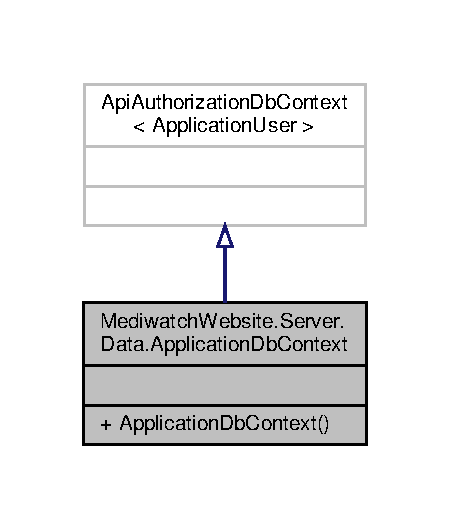
\includegraphics[width=216pt]{class_mediwatch_website_1_1_server_1_1_data_1_1_application_db_context__inherit__graph}
\end{center}
\end{figure}


Graphe de collaboration de Mediwatch\+Website.\+Server.\+Data.\+Application\+Db\+Context\+:
\nopagebreak
\begin{figure}[H]
\begin{center}
\leavevmode
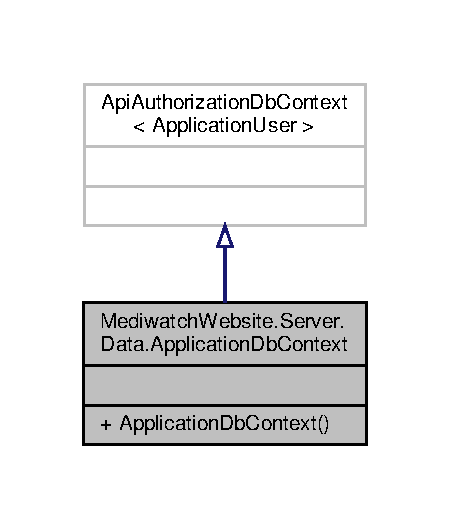
\includegraphics[width=216pt]{class_mediwatch_website_1_1_server_1_1_data_1_1_application_db_context__coll__graph}
\end{center}
\end{figure}
\subsection*{Fonctions membres publiques}
\begin{DoxyCompactItemize}
\item 
\mbox{\Hypertarget{class_mediwatch_website_1_1_server_1_1_data_1_1_application_db_context_a7bfe28d9e655a502f9995126239ed4d7}\label{class_mediwatch_website_1_1_server_1_1_data_1_1_application_db_context_a7bfe28d9e655a502f9995126239ed4d7}} 
{\bfseries Application\+Db\+Context} (Db\+Context\+Options options, I\+Options$<$ Operational\+Store\+Options $>$ operational\+Store\+Options)
\end{DoxyCompactItemize}


La documentation de cette classe a été générée à partir du fichier suivant \+:\begin{DoxyCompactItemize}
\item 
Server/\+Data/Application\+Db\+Context.\+cs\end{DoxyCompactItemize}

\hypertarget{class_mediwatch_website_1_1_server_1_1_data_1_1_migrations_1_1_application_db_context_model_snapshot}{}\section{Référence de la classe Mediwatch\+Website.\+Server.\+Data.\+Migrations.\+Application\+Db\+Context\+Model\+Snapshot}
\label{class_mediwatch_website_1_1_server_1_1_data_1_1_migrations_1_1_application_db_context_model_snapshot}\index{Mediwatch\+Website.\+Server.\+Data.\+Migrations.\+Application\+Db\+Context\+Model\+Snapshot@{Mediwatch\+Website.\+Server.\+Data.\+Migrations.\+Application\+Db\+Context\+Model\+Snapshot}}


Graphe d\textquotesingle{}héritage de Mediwatch\+Website.\+Server.\+Data.\+Migrations.\+Application\+Db\+Context\+Model\+Snapshot\+:
\nopagebreak
\begin{figure}[H]
\begin{center}
\leavevmode
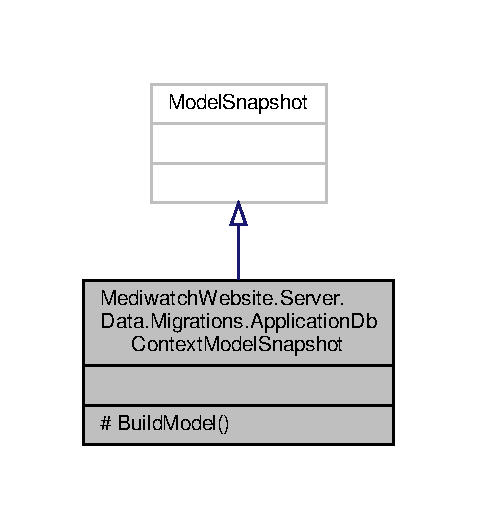
\includegraphics[width=229pt]{class_mediwatch_website_1_1_server_1_1_data_1_1_migrations_1_1_application_db_context_model_snapshot__inherit__graph}
\end{center}
\end{figure}


Graphe de collaboration de Mediwatch\+Website.\+Server.\+Data.\+Migrations.\+Application\+Db\+Context\+Model\+Snapshot\+:
\nopagebreak
\begin{figure}[H]
\begin{center}
\leavevmode
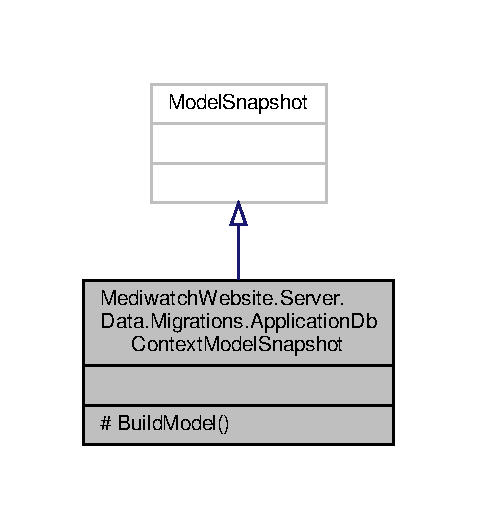
\includegraphics[width=229pt]{class_mediwatch_website_1_1_server_1_1_data_1_1_migrations_1_1_application_db_context_model_snapshot__coll__graph}
\end{center}
\end{figure}
\subsection*{Fonctions membres protégées}
\begin{DoxyCompactItemize}
\item 
\mbox{\Hypertarget{class_mediwatch_website_1_1_server_1_1_data_1_1_migrations_1_1_application_db_context_model_snapshot_a2cb0055d80d12c9613b87de79eb330fb}\label{class_mediwatch_website_1_1_server_1_1_data_1_1_migrations_1_1_application_db_context_model_snapshot_a2cb0055d80d12c9613b87de79eb330fb}} 
override void {\bfseries Build\+Model} (Model\+Builder model\+Builder)
\end{DoxyCompactItemize}


La documentation de cette classe a été générée à partir du fichier suivant \+:\begin{DoxyCompactItemize}
\item 
Server/\+Data/\+Migrations/Application\+Db\+Context\+Model\+Snapshot.\+cs\end{DoxyCompactItemize}

\hypertarget{class_mediwatch_website_1_1_server_1_1_models_1_1_application_user}{}\section{Référence de la classe Mediwatch\+Website.\+Server.\+Models.\+Application\+User}
\label{class_mediwatch_website_1_1_server_1_1_models_1_1_application_user}\index{Mediwatch\+Website.\+Server.\+Models.\+Application\+User@{Mediwatch\+Website.\+Server.\+Models.\+Application\+User}}


Graphe d\textquotesingle{}héritage de Mediwatch\+Website.\+Server.\+Models.\+Application\+User\+:
\nopagebreak
\begin{figure}[H]
\begin{center}
\leavevmode
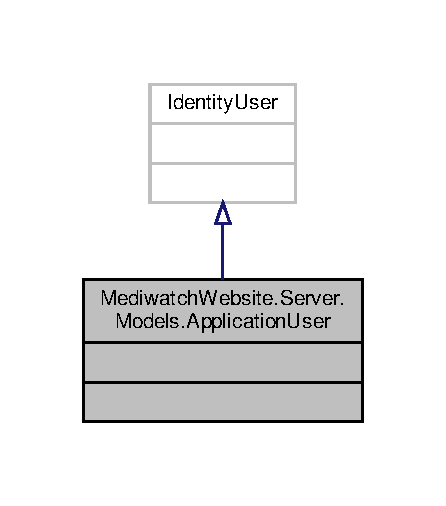
\includegraphics[width=214pt]{class_mediwatch_website_1_1_server_1_1_models_1_1_application_user__inherit__graph}
\end{center}
\end{figure}


Graphe de collaboration de Mediwatch\+Website.\+Server.\+Models.\+Application\+User\+:
\nopagebreak
\begin{figure}[H]
\begin{center}
\leavevmode
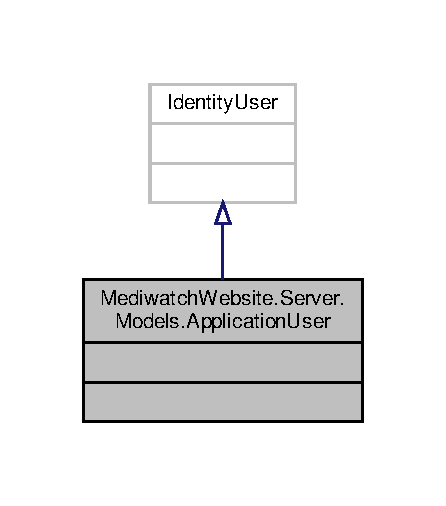
\includegraphics[width=214pt]{class_mediwatch_website_1_1_server_1_1_models_1_1_application_user__coll__graph}
\end{center}
\end{figure}


La documentation de cette classe a été générée à partir du fichier suivant \+:\begin{DoxyCompactItemize}
\item 
Server/\+Models/Application\+User.\+cs\end{DoxyCompactItemize}

\hypertarget{class_mediwatch_website_1_1_server_1_1_data_1_1_migrations_1_1_create_identity_schema}{}\section{Référence de la classe Mediwatch\+Website.\+Server.\+Data.\+Migrations.\+Create\+Identity\+Schema}
\label{class_mediwatch_website_1_1_server_1_1_data_1_1_migrations_1_1_create_identity_schema}\index{Mediwatch\+Website.\+Server.\+Data.\+Migrations.\+Create\+Identity\+Schema@{Mediwatch\+Website.\+Server.\+Data.\+Migrations.\+Create\+Identity\+Schema}}


Graphe d\textquotesingle{}héritage de Mediwatch\+Website.\+Server.\+Data.\+Migrations.\+Create\+Identity\+Schema\+:\nopagebreak
\begin{figure}[H]
\begin{center}
\leavevmode
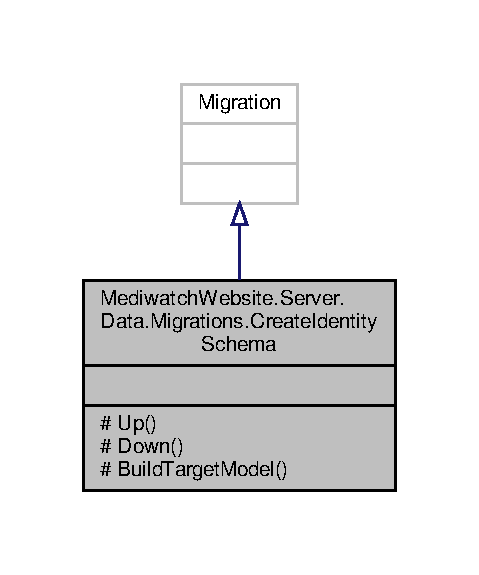
\includegraphics[width=230pt]{class_mediwatch_website_1_1_server_1_1_data_1_1_migrations_1_1_create_identity_schema__inherit__graph}
\end{center}
\end{figure}


Graphe de collaboration de Mediwatch\+Website.\+Server.\+Data.\+Migrations.\+Create\+Identity\+Schema\+:\nopagebreak
\begin{figure}[H]
\begin{center}
\leavevmode
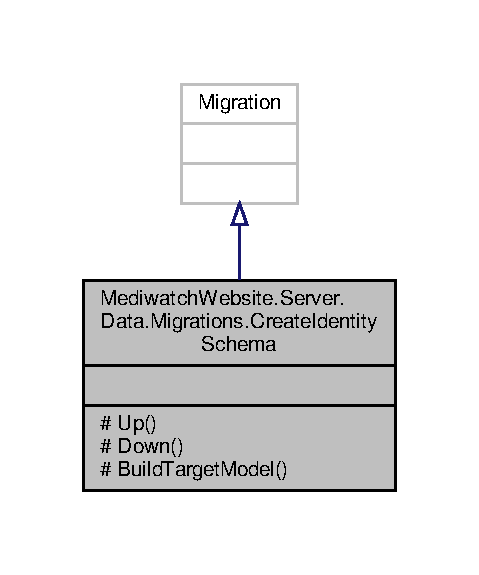
\includegraphics[width=230pt]{class_mediwatch_website_1_1_server_1_1_data_1_1_migrations_1_1_create_identity_schema__coll__graph}
\end{center}
\end{figure}
\subsection*{Fonctions membres protégées}
\begin{DoxyCompactItemize}
\item 
\mbox{\Hypertarget{class_mediwatch_website_1_1_server_1_1_data_1_1_migrations_1_1_create_identity_schema_a8463d6d116a90f1f018b9f8ed60e272a}\label{class_mediwatch_website_1_1_server_1_1_data_1_1_migrations_1_1_create_identity_schema_a8463d6d116a90f1f018b9f8ed60e272a}} 
override void {\bfseries Up} (Migration\+Builder migration\+Builder)
\item 
\mbox{\Hypertarget{class_mediwatch_website_1_1_server_1_1_data_1_1_migrations_1_1_create_identity_schema_adc803467f0ad34f65738416b12b557b7}\label{class_mediwatch_website_1_1_server_1_1_data_1_1_migrations_1_1_create_identity_schema_adc803467f0ad34f65738416b12b557b7}} 
override void {\bfseries Down} (Migration\+Builder migration\+Builder)
\item 
\mbox{\Hypertarget{class_mediwatch_website_1_1_server_1_1_data_1_1_migrations_1_1_create_identity_schema_ae325d871e065f081fc9eada037994d7f}\label{class_mediwatch_website_1_1_server_1_1_data_1_1_migrations_1_1_create_identity_schema_ae325d871e065f081fc9eada037994d7f}} 
override void {\bfseries Build\+Target\+Model} (Model\+Builder model\+Builder)
\end{DoxyCompactItemize}


La documentation de cette classe a été générée à partir des fichiers suivants \+:\begin{DoxyCompactItemize}
\item 
Server/\+Data/\+Migrations/00000000000000\+\_\+\+Create\+Identity\+Schema.\+cs\item 
Server/\+Data/\+Migrations/00000000000000\+\_\+\+Create\+Identity\+Schema.\+Designer.\+cs\end{DoxyCompactItemize}

\hypertarget{class_mediwatch_website_1_1_server_1_1_controllers_1_1_oidc_configuration_controller}{}\section{Référence de la classe Mediwatch\+Website.\+Server.\+Controllers.\+Oidc\+Configuration\+Controller}
\label{class_mediwatch_website_1_1_server_1_1_controllers_1_1_oidc_configuration_controller}\index{Mediwatch\+Website.\+Server.\+Controllers.\+Oidc\+Configuration\+Controller@{Mediwatch\+Website.\+Server.\+Controllers.\+Oidc\+Configuration\+Controller}}


Graphe d\textquotesingle{}héritage de Mediwatch\+Website.\+Server.\+Controllers.\+Oidc\+Configuration\+Controller\+:
\nopagebreak
\begin{figure}[H]
\begin{center}
\leavevmode
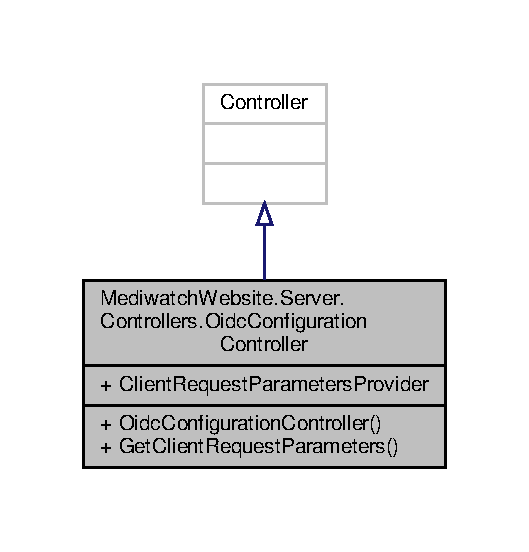
\includegraphics[width=254pt]{class_mediwatch_website_1_1_server_1_1_controllers_1_1_oidc_configuration_controller__inherit__graph}
\end{center}
\end{figure}


Graphe de collaboration de Mediwatch\+Website.\+Server.\+Controllers.\+Oidc\+Configuration\+Controller\+:
\nopagebreak
\begin{figure}[H]
\begin{center}
\leavevmode
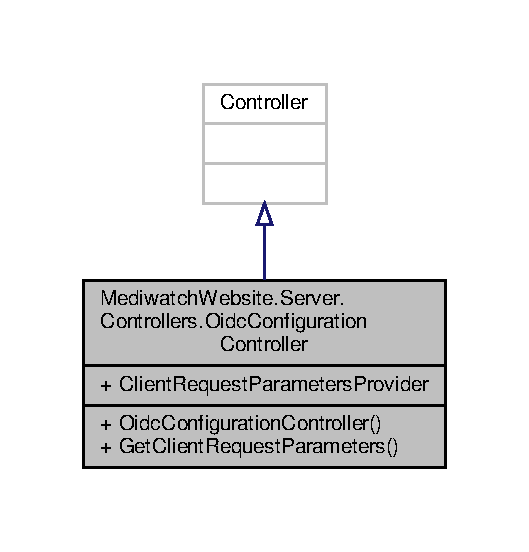
\includegraphics[width=254pt]{class_mediwatch_website_1_1_server_1_1_controllers_1_1_oidc_configuration_controller__coll__graph}
\end{center}
\end{figure}
\subsection*{Fonctions membres publiques}
\begin{DoxyCompactItemize}
\item 
\mbox{\Hypertarget{class_mediwatch_website_1_1_server_1_1_controllers_1_1_oidc_configuration_controller_a8ba9e64456832ebf3dc0dbc74385affb}\label{class_mediwatch_website_1_1_server_1_1_controllers_1_1_oidc_configuration_controller_a8ba9e64456832ebf3dc0dbc74385affb}} 
{\bfseries Oidc\+Configuration\+Controller} (I\+Client\+Request\+Parameters\+Provider client\+Request\+Parameters\+Provider, I\+Logger$<$ \hyperlink{class_mediwatch_website_1_1_server_1_1_controllers_1_1_oidc_configuration_controller}{Oidc\+Configuration\+Controller} $>$ logger)
\item 
\mbox{\Hypertarget{class_mediwatch_website_1_1_server_1_1_controllers_1_1_oidc_configuration_controller_afdb4efd2bdc21800cb6380cb1c8df1bf}\label{class_mediwatch_website_1_1_server_1_1_controllers_1_1_oidc_configuration_controller_afdb4efd2bdc21800cb6380cb1c8df1bf}} 
I\+Action\+Result {\bfseries Get\+Client\+Request\+Parameters} (\mbox{[}From\+Route\mbox{]}string client\+Id)
\end{DoxyCompactItemize}
\subsection*{Propriétés}
\begin{DoxyCompactItemize}
\item 
\mbox{\Hypertarget{class_mediwatch_website_1_1_server_1_1_controllers_1_1_oidc_configuration_controller_adbbef92a4c8f63721c4ee3018103d3db}\label{class_mediwatch_website_1_1_server_1_1_controllers_1_1_oidc_configuration_controller_adbbef92a4c8f63721c4ee3018103d3db}} 
I\+Client\+Request\+Parameters\+Provider {\bfseries Client\+Request\+Parameters\+Provider}\hspace{0.3cm}{\ttfamily  \mbox{[}get\mbox{]}}
\end{DoxyCompactItemize}


La documentation de cette classe a été générée à partir du fichier suivant \+:\begin{DoxyCompactItemize}
\item 
Server/\+Controllers/Oidc\+Configuration\+Controller.\+cs\end{DoxyCompactItemize}

\hypertarget{class_mediwatch_website_1_1_server_1_1_program}{}\section{Référence de la classe Mediwatch\+Website.\+Server.\+Program}
\label{class_mediwatch_website_1_1_server_1_1_program}\index{Mediwatch\+Website.\+Server.\+Program@{Mediwatch\+Website.\+Server.\+Program}}


Graphe de collaboration de Mediwatch\+Website.\+Server.\+Program\+:\nopagebreak
\begin{figure}[H]
\begin{center}
\leavevmode
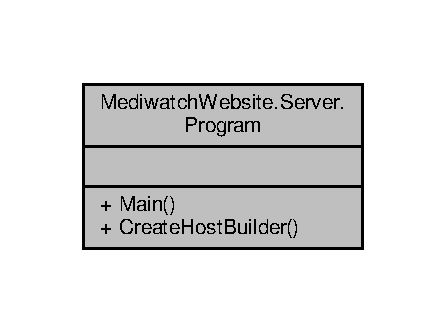
\includegraphics[width=214pt]{class_mediwatch_website_1_1_server_1_1_program__coll__graph}
\end{center}
\end{figure}
\subsection*{Fonctions membres publiques statiques}
\begin{DoxyCompactItemize}
\item 
\mbox{\Hypertarget{class_mediwatch_website_1_1_server_1_1_program_aefcfeb926a88108a29b0f089d7a9f38e}\label{class_mediwatch_website_1_1_server_1_1_program_aefcfeb926a88108a29b0f089d7a9f38e}} 
static void {\bfseries Main} (string\mbox{[}$\,$\mbox{]} args)
\item 
\mbox{\Hypertarget{class_mediwatch_website_1_1_server_1_1_program_abdb5d3ebe00278212ac69d53683e24f1}\label{class_mediwatch_website_1_1_server_1_1_program_abdb5d3ebe00278212ac69d53683e24f1}} 
static I\+Host\+Builder {\bfseries Create\+Host\+Builder} (string\mbox{[}$\,$\mbox{]} args)
\end{DoxyCompactItemize}


La documentation de cette classe a été générée à partir du fichier suivant \+:\begin{DoxyCompactItemize}
\item 
Server/Program.\+cs\end{DoxyCompactItemize}

\hypertarget{class_mediwatch_website_1_1_server_1_1_startup}{}\section{Référence de la classe Mediwatch\+Website.\+Server.\+Startup}
\label{class_mediwatch_website_1_1_server_1_1_startup}\index{Mediwatch\+Website.\+Server.\+Startup@{Mediwatch\+Website.\+Server.\+Startup}}


Graphe de collaboration de Mediwatch\+Website.\+Server.\+Startup\+:
\nopagebreak
\begin{figure}[H]
\begin{center}
\leavevmode
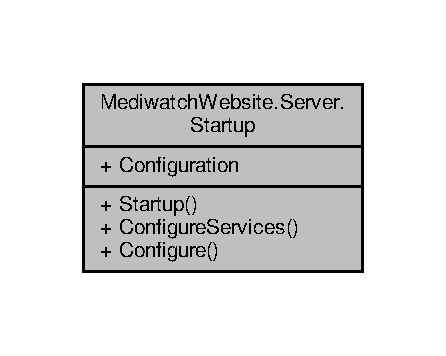
\includegraphics[width=214pt]{class_mediwatch_website_1_1_server_1_1_startup__coll__graph}
\end{center}
\end{figure}
\subsection*{Fonctions membres publiques}
\begin{DoxyCompactItemize}
\item 
\mbox{\Hypertarget{class_mediwatch_website_1_1_server_1_1_startup_ad316a2daabb5739ffe24d385529a2fb7}\label{class_mediwatch_website_1_1_server_1_1_startup_ad316a2daabb5739ffe24d385529a2fb7}} 
{\bfseries Startup} (I\+Configuration configuration)
\item 
\mbox{\Hypertarget{class_mediwatch_website_1_1_server_1_1_startup_abbc6953beb2140feccf70e0ab6e4b12b}\label{class_mediwatch_website_1_1_server_1_1_startup_abbc6953beb2140feccf70e0ab6e4b12b}} 
void {\bfseries Configure\+Services} (I\+Service\+Collection services)
\item 
\mbox{\Hypertarget{class_mediwatch_website_1_1_server_1_1_startup_adca78a113e96adf3237be1a5d92012c0}\label{class_mediwatch_website_1_1_server_1_1_startup_adca78a113e96adf3237be1a5d92012c0}} 
void {\bfseries Configure} (I\+Application\+Builder app, I\+Web\+Host\+Environment env)
\end{DoxyCompactItemize}
\subsection*{Propriétés}
\begin{DoxyCompactItemize}
\item 
\mbox{\Hypertarget{class_mediwatch_website_1_1_server_1_1_startup_a5ff542e1011c165e6eb0035814d6f0ff}\label{class_mediwatch_website_1_1_server_1_1_startup_a5ff542e1011c165e6eb0035814d6f0ff}} 
I\+Configuration {\bfseries Configuration}\hspace{0.3cm}{\ttfamily  \mbox{[}get\mbox{]}}
\end{DoxyCompactItemize}


La documentation de cette classe a été générée à partir du fichier suivant \+:\begin{DoxyCompactItemize}
\item 
Server/Startup.\+cs\end{DoxyCompactItemize}

\hypertarget{class_mediwatch_website_1_1_server_1_1_controllers_1_1_weather_forecast_controller}{}\section{Référence de la classe Mediwatch\+Website.\+Server.\+Controllers.\+Weather\+Forecast\+Controller}
\label{class_mediwatch_website_1_1_server_1_1_controllers_1_1_weather_forecast_controller}\index{Mediwatch\+Website.\+Server.\+Controllers.\+Weather\+Forecast\+Controller@{Mediwatch\+Website.\+Server.\+Controllers.\+Weather\+Forecast\+Controller}}


Graphe d\textquotesingle{}héritage de Mediwatch\+Website.\+Server.\+Controllers.\+Weather\+Forecast\+Controller\+:\nopagebreak
\begin{figure}[H]
\begin{center}
\leavevmode
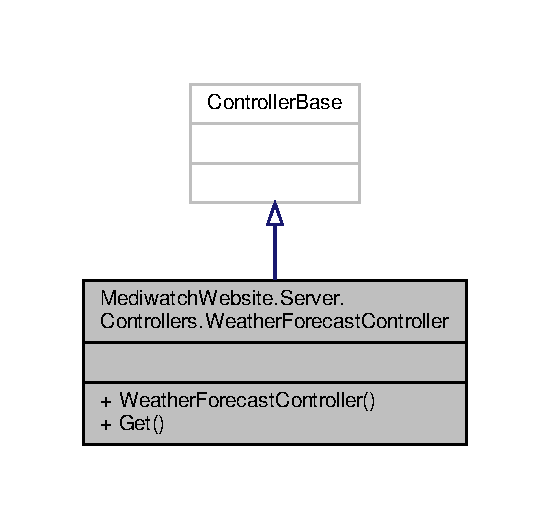
\includegraphics[width=264pt]{class_mediwatch_website_1_1_server_1_1_controllers_1_1_weather_forecast_controller__inherit__graph}
\end{center}
\end{figure}


Graphe de collaboration de Mediwatch\+Website.\+Server.\+Controllers.\+Weather\+Forecast\+Controller\+:\nopagebreak
\begin{figure}[H]
\begin{center}
\leavevmode
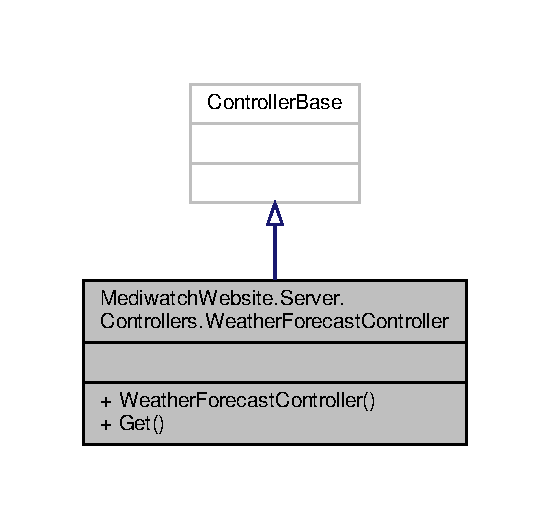
\includegraphics[width=264pt]{class_mediwatch_website_1_1_server_1_1_controllers_1_1_weather_forecast_controller__coll__graph}
\end{center}
\end{figure}
\subsection*{Fonctions membres publiques}
\begin{DoxyCompactItemize}
\item 
\mbox{\Hypertarget{class_mediwatch_website_1_1_server_1_1_controllers_1_1_weather_forecast_controller_a1692c7a64dc181890c1e2215e8f70d97}\label{class_mediwatch_website_1_1_server_1_1_controllers_1_1_weather_forecast_controller_a1692c7a64dc181890c1e2215e8f70d97}} 
{\bfseries Weather\+Forecast\+Controller} (I\+Logger$<$ \hyperlink{class_mediwatch_website_1_1_server_1_1_controllers_1_1_weather_forecast_controller}{Weather\+Forecast\+Controller} $>$ logger)
\item 
\mbox{\Hypertarget{class_mediwatch_website_1_1_server_1_1_controllers_1_1_weather_forecast_controller_a6a1d7d76fd55ecfad8f1bab04e5fa50b}\label{class_mediwatch_website_1_1_server_1_1_controllers_1_1_weather_forecast_controller_a6a1d7d76fd55ecfad8f1bab04e5fa50b}} 
I\+Enumerable$<$ Weather\+Forecast $>$ {\bfseries Get} ()
\end{DoxyCompactItemize}


La documentation de cette classe a été générée à partir du fichier suivant \+:\begin{DoxyCompactItemize}
\item 
Server/\+Controllers/Weather\+Forecast\+Controller.\+cs\end{DoxyCompactItemize}

%--- End generated contents ---

% Index
\backmatter
\newpage
\phantomsection
\clearemptydoublepage
\addcontentsline{toc}{chapter}{Index}
\printindex

\end{document}
